% \documentclass{llncs}
\documentclass[12pt]{article}
\usepackage{sbc-template}
\usepackage[english]{babel}
\usepackage[utf8]{inputenc}
\usepackage{amsmath}
\usepackage{graphicx}
\usepackage{natbib}
\usepackage{subfigure}

% \newcommand{\teamname}{VeRLab\_Rescue~}
\newcommand{\teamname}{RoboCop Brothers~}

\hyphenation{av-a-lanches}

\title{\teamname Team Description Paper}

\author{Anderson Tavares, Elerson Rubens, Hector Azpurua,\\ Levi Vasconcelos, Rafael Colares, Ramon Melo\inst{1}}

\address{VeRLab -- Department of Computer Science \\ Universidade Federal de Minas Gerais
  (UFMG)\\
  Belo Horizonte -- MG -- Brazil
  \email{\{anderson,elerson,hector.azpurua,levi-vasconcelos,rcolares,ramonmelo\}@dcc.ufmg.br}
}

\begin{document}

\maketitle

\begin{abstract}
This paper describes the strategy of \teamname team to the Robocup Rescue Simulator Agents competition. The importance of this type of simulation is to test and improve plans of rescue in disaster environments. Our approach relies on field agents capable of individual decision making, relegating the center agents to an informational role. Our main contributions are the scheme for prediction of fire evolution done by fire brigades, the behaviour-based strategy for police forces and the simple auction-based scheme for recruiting in tasks that demand more than one agent.
\end{abstract}

%%% SECTION: Introduction
\section{Introduction}
\label{sec:intro}

Rescue operations in disaster situations, such as earthquakes, tsunamis, avalanches, for example, are a serious social issue. These operations involve different agents (police forces, firefighters, paramedics, among others) in a hostile environment: buildings collapse, civilians get wounded, streets get blocked, water and power supplies get compromised and communication is limited, making information about the problem scarce and imprecise.

Such situations demand systems that can create robust, dynamic and intelligent search and rescue plans to aid human effort. Within this context, the goal in RoboCup Rescue Agent \& Multi-agent challenge competition is to foster research and development in the field of coordination in multiagent systems. In 2015, the challenge is to program teams of fire brigades, paramedic and police forces in the Agent RoboCup Rescue platform \citep{Kitano2000} and a decentralized constraint optimization problem (DCOP) algorithm in RMASBench \citep{Kleiner+2013}. 

% must coordinate in order to minimize the damage caused in a city by an earthquake.

This paper describes the strategies that will be used to guide \teamname team in  Robocup Rescue Agent \& Multi-agent challenge competition. It is divided in two main parts. In the first part (Section \ref{sec:agent}), we describe our main goals in the Agent competition, which are: to develop a model to predict how the fire evolves in burning buildings, to define a behaviour-based strategy for the police force agents %to use an efficient message compression scheme to save bandwidth in communication 
and to use a simple  method for recruiting in tasks that demand more than one agent. In the second part (Section \ref{sec:multi-agent}), we describe our approach to the multi-agent competition, which involves the implementation of eXtreme-Ants \citep{Santos&Bazzan2009optmas}, a scalable algorithm based on swarm intelligence for task allocation in dynamic environments.


\section{Units' strategies}
\label{sec:strategies}

%%%SUBSECTION: Ambulance team
\section{Ambulance Team}
\label{sec:ambulance}

This team is responsible by the most important task in a disaster environment, namely the search and rescue of injured civilians. Seeking for this goal, the ambulance team will be aided by the other agents with respect to the discovery of new victims.

%The team of paramedics will be divided into sectors, defined by the number of available agents and map size. These regions will have a category of importance measured by the quantity of civilians not rescued yet, ordering the contingent of agents to be designated to most important areas. Separating the agents into regions of interest will make them cover all the map and save, in thesis, the majority of civilians.
% Buscando pela eficiência no resgate, os tipos de paramédicos serão divididos em setores, definidos pela quantidade de agentes deste tipo disponível. Estas regiões serão regidas por um grau de importância medida pela quantidade de civis ainda por serem resgatados naquela área. Isso fará com que o contingente de agentes seja designado para áreas mais interessantes para realização de resgates.

\subsection{Task Allocation}

The task prioritization of this team will be governed by the life estimation of the alive civilians. Life estimation uses the same method of RoboCup Rescue Simulator regarding damage calculation. However, we don't have access to the values of the parameters used by the simulator, thus we use estimated ones.

With life estimation, the ambulance team calculates the priority of the civilian based on the distance between them and whether or not the civilian is in a burning building.

%Based on these features, the agents will tend to save civilians with higher probability of survival. %, lowering the priority of the others civilians with less chance to live.

%upon the circumstances of scenario.
%the life estimation of all targets of rescue. This estimation will take into account the distance between the agent and the task, as well as your life and severity of your injury, if the civilian is inside or not a burning building or if exists some blockage between them. With this values, the agents must incline to civilians with bigger probability of survive. upon the circunstances of scenario.
% A priorização das tarefas dentre a equipe de ambulancias será regida pela estimativa de vida de todos os alvos de resgate. Esta estimativa levará em consideração a distância entre o agente e o mesmo, bem como sua vida e a severidade do ferimento do mesmo, além de se o mesmo se encontra ou não dentro de construções em chamas ou se existem bloqueios entre o caminho do agente e do alvo. Dados estes valores, os agentes devem se inclinar para os civis que tem maior probabilidade de sobrevivencia, mediante as circunstancias do cenário.


%%%SUBSECTION: Police force
\subsection{Police Force}
\label{sec:police}
This team has two main goals: to clear obstructed paths and to scout unvisited areas of the map. The first goal can be divided into three jobs with different priorities, in order: i) clear obstructed paths of important buildings, ii) clear paths that are obstructing other agents, iii) clear random obstructed paths. The second goal is to continuously search the map for survivors and fire spots.
% Divididos em 3 grupos: "fixo", sob demanda e batedor. Fixos limparão caminhos pré-determinados. Sob demanda irão limpar caminhos dos agentes que os chamarem. Batedores irão coletar informações pelo mapa.

To achieve these goals, the police force agents will use a behaviour-based controller. Each agent chooses a behaviour based on its position and the location of important features on the map. The behaviours are:

\begin{itemize}

\item Sweeper: the ``sweeper'' behaviour will try to clear important paths. These paths includes the vicinity of important map features;

\item By-demand: the ``by-demand'' behaviour will clear their own vicinity and will constantly listen to the communication channels for ``help messages'';

\item Scout: the ``scout'' behaviour will keep searching inside buildings for survivors.

\end{itemize}

\subsubsection{Task Allocation}
Initially, the map will be divided into \emph{n} clusters, where \emph{n} is the number of police force team agents. These clusters will be created taking into account the size of the map and the localization of each agent. Agents who are near an important feature of the map will be given the ``sweeper'' behaviour, while agents who are on other areas will be given the ``by-demand'' behaviour. When an agent finishes its tasks, it will then be assigned to the ``scout'' behaviour.

The ``sweeper'' agent task is simple and direct: it will clear its cluster's paths untill all paths are clear. It will not listen to any communication channel or stop its task for any reason. The ``by-demand'' agent task is more complicated, as it will be listening to a communication channel and responding  to help calls. An agent from any other team will be able to broadcast a distress message to the police force team informing that it is trapped and need assistance. This message will contain the sender's current task and location. When a ``by-demand'' agent receives a help message and it is the closest to the sender agent, this ``by-demand'' agent will drop its current task and will respond to that message.

Both behaviours, ``sweeper'' and ``by-demand'', will keep listening to help messages from civillians and will keep searching for fire spots, in order to report these events to the proper agent team. Once they finish their tasks, they will be assigned to the ``scout'' behaviour. Agents with this behaviour will wander through the map helping other police force team agents and searching for survivors and fire spots.
% Inicialmente, existirão apenas fixos e sob demanda. Quando um fixo terminar sua tarefa, ele se torna sob-demanda. Ao longo do tempo, os sob demanda viram batedores.
% Implementar o Q-learning no agente policia
% dividi-los em dois times, um fica responsavel por desbloquear caminhos 'vitais' (até refugio ou hidrantes, por ex.) e outro time escuta os canais dos outros agentes para limpar o caminho deles até suas tarefas.

%\subsubsection{Task Allocation}


%%%SUBSECTION: Fire brigade
\subsection{Fire brigade}
\label{sec:firefighters}
Similarly to the ambulance team and police force, fire brigade agents will be divided in sectors of the map. %The number of sectors depends on map size and number of fire brigades. % on the whole map. 
A score will be assigned to each sector, depending on its importance. For the fire brigades, the importance of a sector depends on the number of burning buildings and the disaster potential of the sector. The disaster potential is related to buried civilians, gas stations and building density of a sector. Building density takes into account the total area (ground area $\times$ number of floors) of all buildings in a sector. We want to prevent fire from spreading to buildings with buried civilians, to gas stations and to areas with high building density.

Firefighters will assign a score to each burning building depending on the ``effort'' needed to extinguish the fire on the building. The effort is related to the amount of water and time required to control the fire on a building. To calculate the effort, we need a model of how fire evolves in a building along time. This model will be given by a regression over the attributes of the building that the fire brigade agent can observe: fieryness, temperature, material and total area.

Data for the regression is extracted from the simulator logs. After several runs on different maps, a significant amount of data from different buildings can be obtained and used as input for the regression.

\subsubsection{Task Allocation}

Firefighters assign a score to each building. The score takes into account the importance of the building (the ones with buried civilians and/or located near gas stations are more important), the agent-to-building distance and effort needed to extinguish the fire. Effort estimation takes as input the prediction of how fire evolves (obtained from the regression model previously discussed) and returns a measure of water and time needed to control the fire. The importance of the building increases its score whereas the distance and the effort decreases its score (a fire brigade agent will prefer to extinguish fires on close, important buildings that do not require too much effort). Figure \ref{fig:firebrigade} shows how a firefighter calculates the score of a building.

\begin{figure}[!ht]
     \centering
     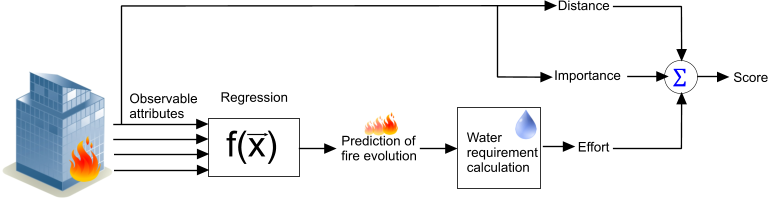
\includegraphics[width=12cm]{img/firebrigade.png}
     \caption{Building score calculation procedure performed by fire brigade agents.}
     \label{fig:firebrigade}
\end{figure}


After deciding which fire to fight, the firefighter calculates whether it is able to extinguish the fire alone. If not, the agent requests help from teammates, using the recruitment method discussed in Section \ref{sec:recruiting}.


%%%SUBSECTION: center
\section{Center agents}
\label{sec:center}
In our strategy, center agents listen to radio communication between agents, accumulating knowledge contained in the messages and replicating important messages to avoid loss of information due to communication unreliability. Using the accumulated knowledge from listening to multiple communication channels, center agents are able to build a more accurate world view. Eventually, center agents send messages to agents in specific channels to give them information previously sent in other channels. This is done in order to make knowledge among agents more uniform.

Center agents do not assign tasks to field agents. Their role is merely informational. The decision of engaging in a task is made individually by each field agent. Therefore, our field agents are autonomous decision-makers. The advantage of this approach is that our strategy does not depend heavily on the center agents. Although their knowledge bases will lack some information provided by the center agents, the decision-making process of our field agents will not change, thus they should not be heavily affected by the absence of center agents.

%Nossa abordagem nao depende fortemente de centrais; elas serao usadas apenas para escutar mais de um canal e replicar/propagar mensagens ``importantes''


\section{Common issues}
\label{sec:common}
% Problemas comuns a todos: temos a compactação de mensagens para a comunicação e o path planning.

%%%SUBSECTION: communication
\subsection{Communication}
\label{sec:communication}

\subsubsection{Message construction}
The goal of communication is to increase the knowledge base of agents and to improve coordination among them. However, in a disaster scenario, communication can be unreliable and bandwidth is limited. To address these problems, our communication strategy is based on a simple protocol. We define three message types for each kind of problem (blockades, burning buildings and buried civilians) the agents may encounter:

\begin{itemize}
 \item Report: the agent found a problem and reports it along with relevant information to its teammates. % Report messages contain information about the problem so that other agents can update their knowledge bases and reason about the recently discovered problem, that is, deciding to engage or not.

 \item Engage: the agent decided to engage in a problem. Engage messages also contain information about the problem so that other agents can update their knowledge bases even if the problem was reported earlier.

 \item Solved: the agent solved the problem and no further action about it is required. %Solved messages do not contain information about the problem status (such as the temperature of a building) since the problem was solved and no further action is needed.
\end{itemize}

Coordination among agents, i.e., requesting help for more effort-demanding tasks require a special protocol, described in Section \ref{sec:recruiting}.

In order to save radio bandwidth and maximize the amount of data shared between the agents, our communication will use a data compression algorithm. Each agent is responsible for compressing/decompressing the communication data.

\subsubsection{Recruiting protocol}
\label{sec:recruiting}
When an agent estimates that it needs help to perform a task, it starts a recruitment process consisting of the following three steps: first, a \msg{request} message is sent by the recruiter agent to other agents. Agents who receive the \msg{request} message and are available to help  send back an \msg{committed} message. Receiving \msg{committed} messages allows the recruiter agent to select the teammates that will help best in the task. \msg{Engage} messages are sent to the selected teammates and \msg{release} messages are sent to non-selected teammates. This process is a simplification of the recruitment protocol of eXtreme-Ants algorithm (Section \ref{sec:multi-agent}). Figure \ref{fig:auction} illustrates the three-step recruitment process.

%It should be noted that messages are always broadcasted in a given channel, that is, all agents can hear all messages in the channel. When it is said that a message is directed to a specific agent, the meaning is that the message is broadcasted in the channel but it has additional information so that non-targets of the message can ignore it.

% Sera implementado um leilão em 3 etapas (anúncio, recebimento de 'ofertas' e recrutamento) para bombeiros pedirem auxílio em tarefas dificeis.
% Compactação


%%%SUBSECTION: path planning
\section{Path planning}
\label{sec:path}

\subsection{Augmented graph}
\label{sec:augraph}
To enhance the basic path planning capabilities provided by the Rescue Simulator's sample agent, we create an augmented neighborhood graph that conveys more information about distance among areas. The augmented graph helps guiding agent navigation and is associated with the Police Force clearing procedures.

In the following discussion, we refer to an area as a building or a road, according to the naming in Rescue Simulator's source code. Besides, two areas are considered neighbors if they are adjacent and an agent can move between them in the absence of blockades.

In the sample search graph (available in the Rescue Simulator package), areas are the nodes and arcs connect neighbor areas. In the augmented graph, a node exists at each door or passage between areas. These nodes are located in the midpoint of the door or passage. Also, an additional node is located at the centroid of each area. Arcs connect all nodes in the same area. 

The augmented graph allows easier and precise computation for its arc weights. The weights are approximated by the euclidean distance between nodes. Weights are more difficult to calculate in the sample search graph as the nodes have no information about position. 
If the area centroid is considered as its location and weight is given by euclidean distance, large errors could occur as the euclidean distance between centroids may diverge greatly from the distance an agent must actually traverse. Manhattan distance would need to consider area orientation or would incur in errors as well. 

Besides more accurate distance calculations, the augmented graph allows more detailed blockade handling: if the path between two adjacent nodes is blocked, we mark only the edge that connects them as impassable. Other edges inside the same area might still be traversable. In the sample search graph, the edges are not associated with positional information, making it difficult to represent detailed blockade information.

%Algorithm \ref{alg:augbuild} shows how the augmented search graph is constructed.
%
%\begin{algorithm}[ht]
%\begin{algorithmic}
%\FORALL{$a \in MapAreas$} 
%\FORALL{$n \in neighbors(a)$} 
%\STATE Insert node at midpoint of $a$-$n$ door/passage
%\ENDFOR
%\STATE Insert node at centroid of $a$
%\ENDFOR
%\end{algorithmic}
%\caption{Augmented graph construction}
%\label{alg:augbuild}
%\end{algorithm}

Figure \ref{fig:graphs} shows sample and augmented graphs. Nodes in the sample search graph have no position al information, but are drawn in area centroid for illustration purposes. %, as they do not convey positional information. 
%The graph is augmented with the squared orange nodes.

\begin{figure}[!ht]
  \centering
  \subfigure[]{
    {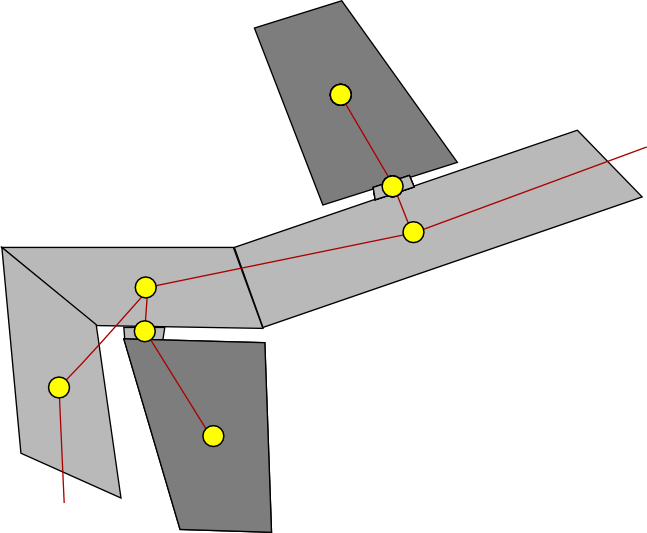
\includegraphics[width=5.2cm]{img/graph-sample.png}}
    \label{fig:sample}
  }
  \subfigure[]{
    {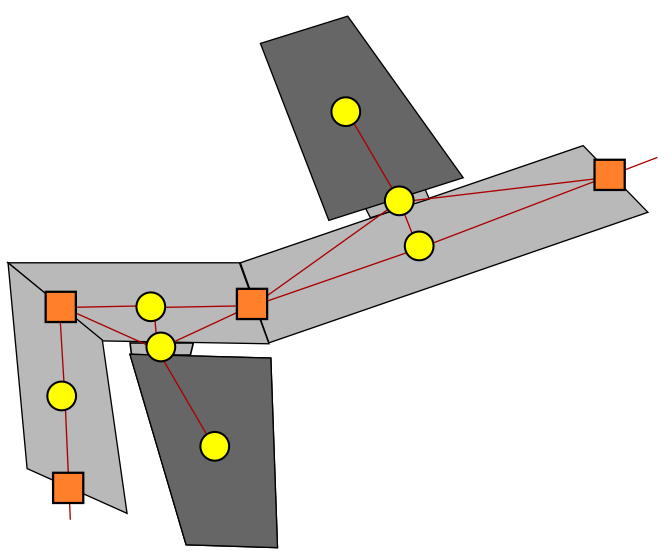
\includegraphics[width=5.2cm]{img/graph-aug.png}}
    \label{fig:aug}
  }%
  \caption{Sample \subref{fig:sample} and augmented \subref{fig:aug} search graphs representing a hypothetical region. Roads are in light gray whereas buildings are in dark gray.}
  \label{fig:graphs}
\end{figure}

Each agent has an instance of the augmented graph. During path planning, an extra node is added at the agent's position. This node is connected to all nodes in the same area, with arc weights assigned via euclidean distance. Path planning proceeds by executing Dijkstra's algorithm with origin as the agent's node and destination as the node at the centroid of the destination area. If the agent wants to move to a specific position in the destination area, a node in that position is temporarily added as well.

For police force agents, the path followed during the clearing process is associated with the augmented graph, as the police force agent clears towards the midpoint of the passage between the current and next area in its path. The midpoints between area's passages corresponds to the nodes added to form the augmented graph (i.e., square nodes in Fig. \ref{fig:aug}).

As a measure for robustness, the search falls back to Breadth First Search (BFS) over the sample search graph if the augmented graph cannot be instantiated. 

%\subsection{Static and dynamic path planning}
%\label{sec:static-dynamic}
%
%Path planning is divided in static and dynamic path planning. Static path planning occurs at the pre-processing stage, where we calculate the shortest path between all pairs of map nodes. %This is done by repeated application of Dijkstra's algorithm. 
%Static path planning generates a table with origin-destination pairs and the route between them. During simulation, agents perform a lookup on this table and save processing time to know the shortest path between two nodes. Static path planning works either with BFS over the sample search graph or Dijkstra over the augmented graph.
%
%Dynamic path planning occurs when a blockade is detected in a road. When this happens, the shortest path between the agent's origin and destination is recalculated. With BFS over the sample search graph, the road is marked as blocked whereas with Dijkstra over the augmented graph, the edges that intersect the blockade are marked as blocked. 
%The new route is updated in the agent's origin-destinations table and a message is sent to other agents to warn them about the blockade. Upon receipt of this kind of message, agents mark the routes containing the blocked road or edges as invalid on their origin-destination table. When the blockade is cleared by police forces, a new message is sent so that the agents can agents mark the routes containing the blocked road or edges as valid again.


%%%SECTION: conclusion
\section{Conclusion}

To address the challenge posed by the agent competition, we present an approach that relies on autonomous decision-making agents. This means that no field or center agent can directly assign a task to other agent. Each agent decides the task it will engage based on its current knowledge, accumulated from observation and communication. Cooperation emerges when agents decide to engage in the same task, or when help is requested via a recruitment method based which is a simplification eXtreme-Ants recruitment process. Even during recruitment, agents are not directly recruited: they can decide whether to offer help to the recruiter or not. The role of center agents is informational, thus in their absence, the decision-making process of field agents does not change.

Our approach relies on map sectorization in order to limit the scope of action of each field agent. The task allocation of field agents is based on the score that they assign to each task, which is associated with the importance and difficulty level of solving the task. We believe that the proposed approach is flexible and robust. Flexibility comes from the fact that the task allocation process for all agents is similar: they assign scores to the tasks that they know and engage in the task with the highest score. Robustness comes from the fact that agents do not depend on each other to decide which task to engage. Thus, the approach can work for several configurations of team sizes and presence of center agents.

For the multi-agent competition, we choose to implement eXtreme-Ants in the RMASBench. The algorithm compares favorably to other E-GAP based approaches in terms of team reward, computational effort and exchanged messages. This implementation represents a scientific contribution as we can establish the first comparison of E-GAP and factor graph-based approaches for task allocation in dynamic environments in a single framework.
%Also, it would be interesting to compare its performance with factor-graph based algorithms, such as max-sum, which is implemented in RMASBench \citep{Kleiner+2013}. For further details of eXtreme-Ants implementation and performance, the reader can refer to \citep{Santos&Bazzan2009optmas}.

%falar das estrategias gerais; resultados esperados
% em suma, nossos agentes sao 'autonomos', isto eh, nao recebem ordem direta de outros agentes, mas deliberam por conta propria se vao realizar as tarefas ou nao

\bibliographystyle{plainnat}
\bibliography{references}

\end{document}
